\documentclass[11pt,a4paper]{article}
\usepackage{cmap}\usepackage[T1]{fontenc}\usepackage[utf8]{inputenc}\usepackage{lmodern}
\usepackage[margin=27mm]{geometry}
\usepackage{amsmath,amssymb,amsthm,mathtools,booktabs,longtable,array,graphicx,microtype}
\usepackage[hidelinks]{hyperref}\usepackage{url}\usepackage[capitalise,noabbrev]{cleveref}
\graphicspath{{../figures/}}
\newtheorem{theorem}{Theorem}[section]
\newtheorem{lemma}[theorem]{Lemma}
\newtheorem{corollary}[theorem]{Corollary}
\newtheorem*{maintheorem}{Theorem}
\providecommand{\tightlist}{\setlength{\itemsep}{0pt}\setlength{\parskip}{0pt}}
\allowdisplaybreaks\emergencystretch=2em
\title{\bfseries History Dirichlet Series of the Nesting Grammar\\[5pt]
\large Factorization, sharp convergence and the growth of generative histories}
\author{UNNS Research Collective}
\date{Research release v001 \quad 26 November 2026}
\begin{document}
\maketitle
\begin{abstract}
Starting from the operation $M\mapsto M(N+1)^2/N$, we study the integer sequences obtained by applying
$x\mapsto x(N+1)^2/N$ whenever $N$ divides $x$, with their ordered words of labels $N$. Each word is possible
exactly from the multiples of a least integer and ends exactly in the multiples of a least endpoint. The Dirichlet
series counting all histories ending at $n$ factors as $\zeta(s)$ times the generating series of least endpoints,
also when depth and source are weighted. Although every fixed depth converges for $\operatorname{Re}s>1/2$,
the full series has abscissa of absolute convergence $\sigma_c=1.5463810\ldots$, the root of
$\sum_{N\ge1}(N/(N+1)^2)^{\sigma}=1$. The histories issuing from any single integer already grow like
$X^{\sigma_c+o(1)}$ up to endpoint $X$. At depth two the series continues meromorphically to
$\operatorname{Re}s>1/3$ with a double pole at $1/2$, and the number of two-letter words with least endpoint
at most $X$ is asymptotic to $\frac{\kappa}{2}\sqrt X\log X$ for an explicit Euler product
$\kappa\approx1.8536$. The series admits no ordinary Euler product. Comparisons with other multiplicative
grammars show which arithmetic hypothesis drives the boundary.
\end{abstract}
\tableofcontents
\section{Introduction}
Fix the generating operation $M\perp N=M(N+1)^2/N$ and continue it on integers: the letter $N$ may be applied
to $x$ when $N\mid x$. From $x=1$ only the letter $1$ is possible and leads to $4$; from $4$ the letters
$1,2,4$ are possible, and so on. Two different words may reach the same integer, and the order of the letters
matters for the sources from which they are possible. The record of a word is
$\mathcal R(w)=(w,K(w),Q(w),E(w))$: the word, its least source, its multiplier and its least endpoint.
Dirichlet series appear here as summaries of these records; the records themselves, including the order of the
letters, remain the underlying object.

\begin{figure}[htbp]\centering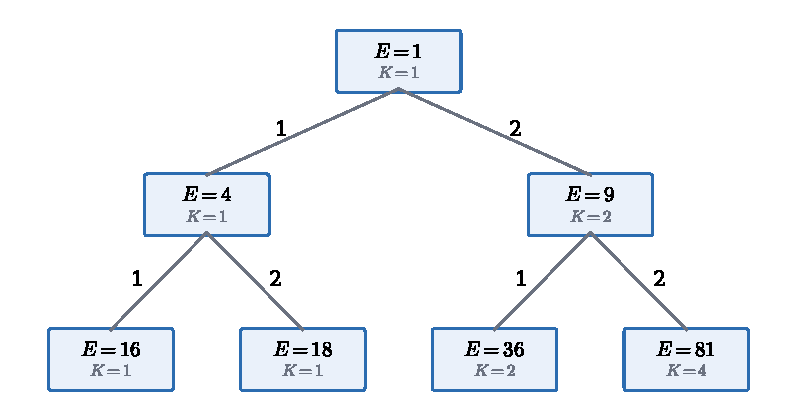
\includegraphics[width=.92\textwidth]{fig_tree.pdf}
\caption{Words over the letters $1$ and $2$ up to length two, with least endpoint $E$ and least source $K$.
Edge labels are the letters.}\label{fig:tree}\end{figure}

\subsection*{Main results}
Write $\mathcal G(s,t)=\sum_wt^{|w|}E(w)^{-s}$ and $B(\sigma)=\sum_{N\ge1}(N/(N+1)^2)^{\sigma}$.
\begin{itemize}
\item \emph{Factorization} (\cref{thm:factor,thm:allhist}). The series of histories ending at $n$ equals
$\zeta(s)\mathcal G(s,t)$; the series over all histories weighted by source and endpoint is again a zeta factor
times a series over words.
\item \emph{Sharp boundary} (\cref{thm:sharp,thm:region}). The $k$-letter sum $G_k(\sigma)$ satisfies
$G_k(\sigma)^{1/k}\to B(\sigma)$; hence $\mathcal G(s,t)$ converges absolutely for $|t|B(\operatorname{Re}s)<1$,
$\operatorname{Re}s>1$, and not when the inequality is reversed.
\item \emph{Growth from one source} (\cref{thm:growth}). The number of histories from any fixed integer with
endpoint at most $X$ is $X^{\sigma_c+o(1)}$.
\item \emph{Fixed depth} (\cref{thm:fixed,thm:depth2}). Every $G_k$ with $k\ge1$ has abscissa $1/2$; $G_2$ has
an explicit continuation and a double pole there.
\end{itemize}

\subsection*{Relation to earlier work}
The least source and least endpoint of a word, the predecessor structure, and the decomposition of history sets
by endpoint are established in the monograph \cite{monograph}, in particular its Lemma~4.2, Proposition~5.5 and
Theorem~19.2; the surrounding source collection is public \cite{sources,index}. The present work adds the depth
and source weighted analytic series, their convergence boundaries, the growth theorem and the depth-two
analysis. The lemma that every prime is reached from the source $1$ proceeds by induction on primes, a device
also used for rational completeness in \cite{algebraic}. Priority with respect to the wider literature has not
been surveyed.

This report is release v001 of the investigation ANS-I of the research programme \emph{Analytic Structures of
the UNNS Substrate}; \cref{sec:register} relates its statements to the programme register. All statements called
theorems, lemmas or corollaries have proofs below; numerical statements are confined to \cref{sec:comp} and are
labelled as computations.
\section{Generation}

The generating operation is the nesting \(M\perp N=M(N+1)^2/N\). A
transition \(T_N(x)=r_Nx\), \(r_N=(N+1)^2/N\), is admissible at an
integer \(x\ge1\) exactly when \(N\mid x\). A \emph{history} is an
admissible sequence
\(x_0\xrightarrow{N_1}x_1\to\cdots\xrightarrow{N_k}x_k\); its ordered
label word is \(w=(N_1,\dots,N_k)\).

Several statements hold for every \emph{integral-image grammar}: labels
\(b\) with multipliers \(r_b=p_b/q_b>1\), \(\gcd(p_b,q_b)=1\), the step
\(x\mapsto r_bx\) being admissible iff \(q_b\mid x\). For the nesting
grammar \(p_N=(N+1)^2\) and \(q_N=N\). We assume the finiteness
condition

\textbf{(F)} every integer is divisible by \(p_b\) for only finitely
many labels \(b\).

The nesting grammar satisfies (F). Write \(Q(w)=\prod_i r_{N_i}\) for
the multiplier of a word.

\subsection{Source and endpoint
evolution}

\begin{theorem}\label{thm:evolution}
For every word \(w\) there are integers \(K(w),E(w)=K(w)Q(w)\) such that
\(w\) is admissible exactly from the sources \(K(w)\mathbb Z_{>0}\),
with endpoints exactly \(E(w)\mathbb Z_{>0}\). Starting from \(K=E=1\)
for the empty word,
\[E(wb)=\frac{p_b\,E(w)}{\gcd(E(w),q_b)},\qquad K(wb)=\frac{q_b\,K(w)}{\gcd(E(w),q_b)} .\]
For nesting, \(E(wN)=(N+1)^2E(w)/\gcd(E(w),N)\) and
\(K(wN)=N\,K(w)/\gcd(E(w),N)\).

\end{theorem}

\begin{proof}

Induction on the length. A source admits \(wb\) iff it admits \(w\) and
the endpoint \(y\in E(w)\mathbb Z_{>0}\) is divisible by \(q_b\), that
is \(y\in L\,\mathbb Z_{>0}\) with \(L=\operatorname{lcm}(E(w),q_b)\).
The new endpoints are \(r_by\in (p_bL/q_b)\mathbb Z_{>0}\) and
\(p_bL/q_b=p_bE(w)/\gcd(E(w),q_b)\). The sources are
\(y/Q(w)\in(L/Q(w))\mathbb Z_{>0}\), and
\(L/Q(w)=K(w)L/E(w)=K(w)q_b/\gcd(E(w),q_b)\).

\end{proof}

The existence of the least source and least endpoint is \cite[Lemma~4.2]{monograph} for the nesting grammar; the recurrences give them letter by letter.

\begin{corollary}[Histories ending at \(n\)]\label{cor:words}
Let \(\mathcal W(n)=\{w:E(w)\mid n\}\). Then \(\mathcal W(n)\) is the
set of words of histories ending at \(n\),
\[\mathcal W(n)=\{\varepsilon\}\ \sqcup\bigsqcup_{b:\;p_b\mid n}\mathcal W\!\left(\tfrac{nq_b}{p_b}\right)b,\]
and under (F) it is finite.

\end{corollary}

\begin{proof}

The first statement is the theorem. A history ends at \(n\) with last
letter \(b\) iff \(n=r_bx\) with \(q_b\mid x\), which holds for an
integer \(x\) iff \(p_b\mid n\), and then \(x=nq_b/p_b<n\). Finiteness
follows by strong induction on \(n\).

\end{proof}

\subsection{Prime-coordinate
evolution}

\begin{theorem}\label{thm:prime}
A nesting transition acts by \(v_p(T_N(x))=v_p(x)+2v_p(N+1)-v_p(N)\).
For minimal endpoints, \(e_p(w)=v_p(E(w))\) satisfies
\[e_p(wN)=2v_p(N+1)+\max\{e_p(w)-v_p(N),\,0\},\] and, with
\(u_i=2v_p(N_i+1)\) and \(d_i=v_p(N_i)\), for \(k\ge1\)
\[e_p(N_1\cdots N_k)=\max_{1\le j\le k}\Big(\sum_{i=j}^{k}u_i-\sum_{i=j+1}^{k}d_i\Big).\]
For each \(p\) at most one of \(v_p(N)\), \(v_p(N+1)\) is non-zero.

\end{theorem}

\begin{proof}

The first two identities are the \(p\)-adic valuations of \(T_N(x)\) and
of the recurrence of \cref{thm:evolution}. For the closed form,
\(e_k=\max\{u_k,\;u_k-d_k+e_{k-1}\}\) with \(e_1=u_1\); substituting the
formula for \(e_{k-1}\) gives the maximum over \(j\le k-1\), and the
term \(u_k\) is the case \(j=k\). The last statement is
\(\gcd(N,N+1)=1\).

\end{proof}

\section{Factorization}

Let \(H_k(n)=\#\{w\in\mathcal W(n):|w|=k\}\) and
\(a_k(n)=\#\{w:|w|=k,\ E(w)=n\}\), and put
\[\mathcal G(s,t)=\sum_w\frac{t^{|w|}}{E(w)^s},\qquad \mathcal Z_H(s,t)=\sum_{n,k}\frac{H_k(n)t^k}{n^s}.\]

\subsection{History factorization and depth-resolved
inversion}

\begin{theorem}\label{thm:factor}
For every integral-image grammar with (F),
\[H_k(n)=\sum_{d\mid n}a_k(d),\qquad a_k(n)=\sum_{d\mid n}\mu(d)H_k(n/d),\]
and, for \(t\ne0\), \(\mathcal Z_H(s,t)\) converges absolutely iff
\(\operatorname{Re}s>1\) and
\(\mathcal G(\operatorname{Re}s,|t|)<\infty\); there
\(\mathcal Z_H(s,t)=\zeta(s)\,\mathcal G(s,t)\).

\end{theorem}

\begin{proof}

Group the words of \(\mathcal W(n)\) by their minimal endpoint
\(d\mid n\) and invert. For the series, with non-negative terms and
\(\sigma=\operatorname{Re}s\),
\[\sum_{n,k}\frac{H_k(n)|t|^k}{n^{\sigma}}=\sum_w|t|^{|w|}\sum_{m\ge1}\frac1{(mE(w))^{\sigma}}=\zeta(\sigma)\,\mathcal G(\sigma,|t|),\]
and the same rearrangement with complex terms gives the identity.

\end{proof}

At \(t=1\) and at the level of coefficients this is the endpoint
decomposition of \cite[Theorem~19.2]{monograph}; the depth grading and the
analytic statement are added here.

\subsection{Factorization of all actual
histories}

Let
\(\mathcal F(s,u,t)=\sum_w t^{|w|}E(w)^{-s}K(w)^{-u}=\sum_wt^{|w|}Q(w)^{-s}K(w)^{-(s+u)}\).

\begin{theorem}\label{thm:allhist}
Summing over all actual histories, given by a source \(x\) and an
admissible word \(w\) with endpoint \(y=Q(w)x\),
\[\sum_{(x,w)}\frac{t^{|w|}}{x^{u}\,y^{s}}=\zeta(s+u)\,\mathcal F(s,u,t)\]
wherever the left side converges absolutely, which for \(t\ne0\) means
\(\operatorname{Re}(s+u)>1\) and absolute convergence of \(\mathcal F\).
On the anti-diagonal, for \(\operatorname{Re}s>1\) and
\(|t|B(\operatorname{Re}s)<1\),
\[\mathcal F(s,-s,t)=\frac1{1-t\sum_b r_b^{-s}},\qquad B(\sigma)=\sum_br_b^{-\sigma}.\]

\end{theorem}

\begin{proof}

By \cref{thm:evolution} the histories with word \(w\) are \(x=mK(w)\), \(y=mE(w)\),
\(m\ge1\); sum over \(m\) first. At \(u=-s\) the weight
\(E^{-s}K^{s}=Q^{-s}\) is multiplicative over letters.

\end{proof}

\(\mathcal G(s,t)=\mathcal F(s,0,t)\). The factorization
\(\mathcal Z_H=\zeta\,\mathcal G\) is the case \(u=0\). Each of these
functions aggregates the records \(\mathcal R(w)=(w,K(w),Q(w),E(w))\):
the distinct words \((1,3)\) and \((3,1)\) both have depth \(2\),
\(K=3\) and \(E=64\), so \(\mathcal F\) does not separate them although
their state sequences \(3\to12\to64\) and \(3\to16\to64\) differ.

\section{Convergence of the nesting
grammar}

From here the grammar is the nesting grammar,
\(B(\sigma)=\sum_{N\ge1}\big(N/(N+1)^2\big)^{\sigma}\) (finite iff
\(\sigma>1\)), and \(B_M\) is the partial sum over \(N\le M\).

\subsection{Sufficient criterion}

\begin{theorem}\label{thm:suff}
If \(\operatorname{Re}s=a>1\), \(\operatorname{Re}(s+u)=b\ge0\) and
\(|t|B(a)<1\), then \(\mathcal F(s,u,t)\) converges absolutely. Also
\(B(2)=\zeta(2)-2\zeta(3)+\zeta(4)<1\).

\end{theorem}

\begin{proof}

\(K(w)\ge1\), so \(\sum_w|t|^{|w|}Q^{-a}K^{-b}\le\sum_k(|t|B(a))^k\).
With \(m=N+1\), \((m-1)^2/m^4=m^{-2}-2m^{-3}+m^{-4}\); also
\(B(2)<\sum_{m\ge3}m^{-2}<1\) because \(r_N>N+2\).

\end{proof}

\subsection{Source-one generation}

\begin{lemma}[Every prime is reached from source 1]\label{lem:primes}
For each prime \(p\) there is a word \(w_p\) admissible from \(1\) with
\(p\mid Q(w_p)\).

\end{lemma}

\begin{proof}

Take \(w_2=(1)\). For \(p>2\) write \(p-1=\prod q^{f_q}\) with \(q<p\),
and concatenate \(f_q\) copies of each \(w_q\). A word admissible from
\(1\) is admissible from every integer, so concatenations of such words
are admissible from \(1\) and their multipliers, which are integers,
multiply. The state reached is divisible by \(p-1\); applying the letter
\(p-1\) gives a state divisible by \(p^2\).

\end{proof}

\begin{lemma}[Saturation]\label{lem:saturation}
Fix \(\sigma\ge0\) and \(M\), and let the letters of
\(v=(v_1,v_2,\dots)\) be independent with law
\(\nu(N)=r_N^{-\sigma}/B_M(\sigma)\), \(N\le M\). There is a word
\(w_0\), admissible from \(1\), such that with probability at least
\(1/2\) the whole infinite word \(w_0v\) is admissible from \(1\).

\end{lemma}

\begin{proof}

For a prime \(p\le M\) let \(X_p(N)=2v_p(N+1)-v_p(N)\). For each power
\(q=p^j\), the map \(N=mq\mapsto mq-1\) sends multiples of \(q\) in
\([1,M]\) injectively to integers \(N'\in[1,M]\) with \(q\mid N'+1\),
and \(\nu(N')\ge\nu(N)\) because \(r_N\) increases. Summing over \(j\)
gives \(\mathbb E\,v_p(N+1)\ge\mathbb E\,v_p(N)\), hence
\[\mathbb E\,X_p\ge\mathbb E\,v_p(N+1)\ge\nu(p-1)>0 .\] The partial sums
\(S_p(k)=\sum_{i\le k}X_p(v_i)\) therefore tend to \(+\infty\) almost
surely, so there is \(C\) with
\(\Pr\{\min_{k\ge0}S_p(k)\ge-C\ \text{for all }p\le M\}\ge1/2\). Let
\(D_p=\max_{N\le M}v_p(N)\) and let \(w_0\) concatenate \(C+D_p\) copies
of \(w_p\) for every \(p\le M\); then \(v_p(Q(w_0))\ge C+D_p\). On the
event above, if the first \(i-1\) letters of \(v\) have been applied,
the state \(x\) has \(v_p(x)=v_p(Q(w_0))+S_p(i-1)\ge D_p\) for every
\(p\le M\), so \(v_i\mid x\).

\end{proof}

The drift \(\mathbb E[2v_p(N+1)-v_p(N)]>0\) is the arithmetic content:
nesting by \(N\) returns the square of \(N+1\) for one factor of \(N\),
and long histories accumulate enough divisibility to admit every later
letter.

\subsection{Exponential growth in depth and the sharp
boundary}

\begin{theorem}\label{thm:sharp}
Let \(G_k(\sigma)=\sum_{|w|=k}E(w)^{-\sigma}\). Then
\(\lim_{k\to\infty}G_k(\sigma)^{1/k}=B(\sigma)\) for \(\sigma>1\), and
the limit is \(+\infty\) for \(0\le\sigma\le1\).

\end{theorem}

\begin{proof}

\(E\ge Q\) gives \(G_k\le B^k\). Call \(v\in\{1..M\}^k\) \emph{good} if
\(w_0v\) is admissible from \(1\). Then \(K(w_0v)=1\), so
\(E(w_0v)=Q(w_0v)\), and
\[G_{|w_0|+k}(\sigma)\ge Q(w_0)^{-\sigma}\sum_{v\ \mathrm{good}}Q(v)^{-\sigma}=Q(w_0)^{-\sigma}B_M(\sigma)^k\,\nu(\mathrm{good})\ge\tfrac12Q(w_0)^{-\sigma}B_M(\sigma)^k .\]
Hence \(\liminf G_k^{1/k}\ge B_M(\sigma)\) for every \(M\).

\end{proof}

\subsection{The region of absolute
convergence}

\begin{theorem}\label{thm:region}
Let \(t\ne0\), \(a=\operatorname{Re}s\) and
\(b=\operatorname{Re}(s+u)\).

\begin{enumerate}
\def\labelenumi{\arabic{enumi}.}
\tightlist
\item
  If \(a\le1\), or if \(a>1\) and \(|t|B(a)>1\), then
  \(\mathcal F(s,u,t)\) does not converge absolutely, for any real
  \(b\).
\item
  If \(b\ge0\), \(a>1\) and \(|t|B(a)<1\), it converges absolutely.
\item
  The series over all actual histories in \cref{thm:allhist} converges absolutely if
  \(b>1\), \(a>1\), \(|t|B(a)<1\); it does not if \(b\le1\), or
  \(a\le1\), or \(a>1\) and \(|t|B(a)>1\).
\end{enumerate}

\end{theorem}

\begin{proof}

\begin{enumerate}
\def\labelenumi{(\arabic{enumi})}
\tightlist
\item
  For \(a\ge0\) choose \(M\) with \(|t|B_M(a)>1\); this is possible in
  both cases since \(B_M(a)\to\infty\) for \(a\le1\). The words with
  \(K=1\) carry no factor of \(b\), and the estimate of \cref{thm:sharp} shows that
  their contribution already diverges. For \(a<0\) each term is at least
  the corresponding term at \(a=0\). (2) is \cref{thm:suff}. (3) combines (1), (2)
  and the factor \(\zeta(b)\).
\end{enumerate}

\end{proof}

The source weight \(K^{-b}\), \(b\ge0\), therefore does not move the
exponential boundary. The surface \(|t|B(a)=1\) itself is not decided
here.

\begin{corollary}[Abscissa]\label{cor:abscissa}
\(\mathcal G(s,1)\) and \(\mathcal Z_H(s,1)\) have abscissa of absolute
convergence \(\sigma_c\), the unique root of
\[\sum_{N\ge1}\Big(\frac{N}{(N+1)^2}\Big)^{\sigma_c}=1,\qquad\sigma_c=1.5463810\ldots\]
Because the coefficients are non-negative, \(s=\sigma_c\) is a singular
point of both series (Landau's theorem \cite[Chapter~11]{apostol}).

\end{corollary}

\begin{proof}

\(B\) decreases continuously from \(+\infty\) (as \(\sigma\to1^+\)) to
\(B(2)<1\). Apply \cref{thm:region} with \(u=0\), and \cref{thm:factor}. Since \(\sigma_c>1\), the
factor \(\zeta(s)\) does not change the abscissa. The decimal value is a
floating-point evaluation with an explicit two-sided tail bound.

\end{proof}
\begin{figure}[htbp]\centering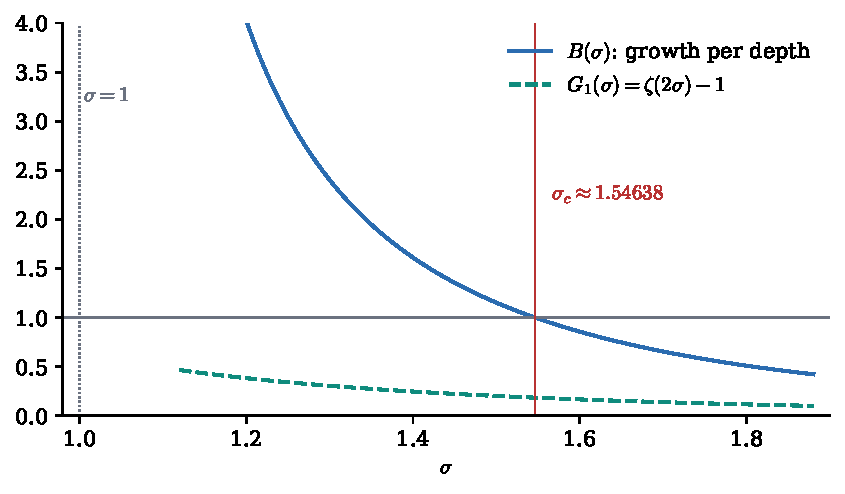
\includegraphics[width=.86\textwidth]{fig_pressure.pdf}
\caption{The growth factor $B(\sigma)$ per letter crosses $1$ at $\sigma_c$, while a single letter, $G_1$, is finite for all $\sigma>1/2$.}\label{fig:pressure}\end{figure}


\subsection{Growth of generative
histories}

For a source \(x\) let \(N_x(X)\) be the number of histories from \(x\)
with endpoint at most \(X\). Let \(A(X)=\#\{w:E(w)\le X\}\) and
\(C(X)=\sum_{n\le X}\#\mathcal W(n)\).

\begin{theorem}\label{thm:growth}
For every source \(x\ge1\),
\[\lim_{X\to\infty}\frac{\log N_x(X)}{\log X}=\lim\frac{\log A(X)}{\log X}=\lim\frac{\log C(X)}{\log X}=\sigma_c .\]

\end{theorem}

\begin{proof}

Upper bounds: for \(\sigma>\sigma_c\), \(N_x(X)\) and \(A(X)\) are at
most
\(\#\{w:Q(w)\le X\}\le\sum_w(X/Q(w))^{\sigma}=X^{\sigma}/(1-B(\sigma))\),
and
\(C(X)=\sum_{E(w)\le X}\lfloor X/E(w)\rfloor\le X^{\sigma}\mathcal G(\sigma,1)\).

Lower bounds: words admissible from \(1\) are admissible from \(x\) and
have \(E=Q\), so \(N_x(X)\ge N_1(X/x)\) and \(N_1(X)\le A(X)\le C(X)\).
Fix \(\alpha<\sigma_c\), choose \(M\) with \(B_M(\alpha)>1\), and let
\(\alpha_M\in(\alpha,\sigma_c)\) solve \(B_M(\alpha_M)=1\). Take \(\nu\)
at \(\sigma=\alpha_M\), let \(\lambda=\sum_{N\le M}\nu(N)\log r_N>0\),
fix \(\varepsilon\in(0,1/2)\) and put
\(k=\lfloor(1-\varepsilon)\log X/\lambda\rfloor\). By the law of large
numbers, with probability tending to \(1\) a word \(v\) of length \(k\)
satisfies
\((1-2\varepsilon)\log X\le\log Q(v)\le(1-\varepsilon/2)\log X\). By
saturation, for large \(X\) the words that are also good have
probability at least \(1/3\). Each such \(v\) has
\(\nu(v)=Q(v)^{-\alpha_M}\le X^{-(1-2\varepsilon)\alpha_M}\), so there
are at least \(X^{(1-2\varepsilon)\alpha_M}/3\) of them, and
\(Q(w_0v)\le X\) for large \(X\). Let \(\varepsilon\to0\) and
\(\alpha\to\sigma_c\).

\end{proof}

In words: the forward history tree of any single integer, already that
of \(1\), grows with the same exponent as the whole architecture, and
that exponent is fixed by the nesting multipliers.

\section{Fixed depth}

\subsection{Convergence at fixed
depth}

\begin{theorem}\label{thm:fixed}
Let \(k\ge1\), \(a>0\), \(b\ge0\) and
\(F_k(a,b)=\sum_{|w|=k}Q(w)^{-a}K(w)^{-b}\). Then \(F_k(a,b)<\infty\)
iff \(a+b>1\) when \(b>0\), and iff \(a>1\) when \(b=0\). In particular
\(G_k(\sigma)=F_k(\sigma,\sigma)\) has abscissa exactly \(1/2\) for
every \(k\ge1\).

\end{theorem}

\begin{proof}

For \(b=0\), \(F_k=B(a)^k\). Let \(b>0\). Divergence for \(a+b\le1\):
the words \((N,1,\dots,1)\) have \(K=N\) and \(Q=r_N4^{k-1}\), so their
terms are of order \(N^{-a-b}\). Convergence: by \cref{thm:evolution}, \(K(wN)=K(w)N/g\)
with \(g=\gcd(E(w),N)\), and \(r_N\ge N\), so
\[\sum_Nr_N^{-a}\Big(\frac gN\Big)^{b}\le\sum_N\frac{g^{b}}{N^{a+b}}\le\sum_{d\mid E(w)}d^{b}\sum_{d\mid N}N^{-a-b}=\zeta(a+b)\sum_{d\mid E(w)}d^{-a}\le\zeta(a+b)\,\tau(E(w)).\]
Since \(\tau(E)\le C_\eta E^{\eta}=C_\eta Q^{\eta}K^{\eta}\), we get
\(F_{k+1}(a,b)\le C_\eta\,\zeta(a+b)\,F_k(a-\eta,b-\eta)\). Choose
\(\eta\) small compared with \(a/k\), \(b/k\) and \((a+b-1)/(2k)\) and
induct from \(F_0=1\).

\end{proof}
\begin{figure}[htbp]\centering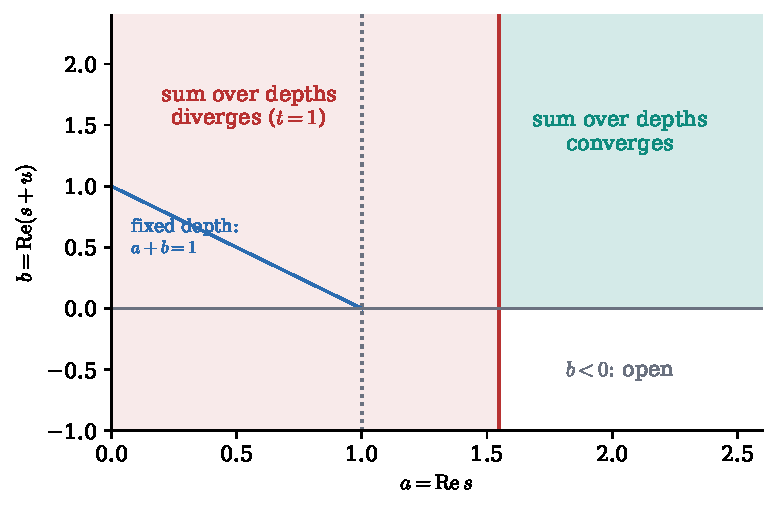
\includegraphics[width=.74\textwidth]{fig_region.pdf}
\caption{Source-weighted series at $t=1$, $a=\operatorname{Re}s$, $b=\operatorname{Re}(s+u)$. The full series changes behaviour at $a=\sigma_c$ for $b\ge0$; each fixed depth $k\ge1$ converges, for $a>0$, $b>0$, exactly above the line $a+b=1$.}\label{fig:region}\end{figure}


Every single depth converges down to \(1/2\), while the sum over depths
stops at \(\sigma_c>3/2\): the boundary is produced by the accumulation
of depth. In the interval \(1/2<\sigma\le1\) all coefficients of
\(\mathcal G(\sigma,t)\) are finite and its radius of convergence in
\(t\) is zero.

\subsection{Depth two}

\begin{theorem}\label{thm:depth2}
\(G_1(s)=\zeta(2s)-1\) and
\[G_2(s)=\sum_{a,b\ge1}\left[\frac{\gcd((a+1)^2,b)}{(a+1)^2(b+1)^2}\right]^{s}.\]
With \(J_s(d)=\sum_{e\mid d}\mu(e)(d/e)^s\),
\(c(d)=\prod_pp^{\lceil v_p(d)/2\rceil}\) and the Hurwitz zeta function
\(\zeta(\cdot,\cdot)\),
\[G_2(s)=\sum_{d\ge1}\frac{J_s(d)}{d^{2s}}\,\zeta\!\left(2s,1+\tfrac1d\right)\Big(\frac{\zeta(2s)}{c(d)^{2s}}-[d=1]\Big).\]
The right side continues \(G_2\) meromorphically to
\(\operatorname{Re}s>1/3\) with a single pole, at \(s=1/2\), of order
two, and \(G_2(s)\sim\dfrac{\kappa}{4(s-1/2)^2}\), where
\[\kappa=\prod_p\Big(1+(1-p^{-1/2})\sum_{j\ge1}p^{-j/2-\lceil j/2\rceil}\Big)\approx1.8536 .\]
Consequently the number of depth-two words with minimal endpoint at most
\(X\) satisfies \[A_2(X)\sim\frac{\kappa}{2}\sqrt X\log X .\]

\end{theorem}

\begin{proof}

The double sum is \cref{thm:evolution}. Expand
\(\gcd(\cdot,\cdot)^s=\sum_{d\mid\gcd}J_s(d)\). Here \(d\mid m^2\) iff
\(c(d)\mid m\), so
\(\sum_{m\ge2,\,d\mid m^2}m^{-2s}=c(d)^{-2s}\zeta(2s)-[d=1]\), and
\(\sum_{d\mid b}(b+1)^{-2s}=d^{-2s}\zeta(2s,1+1/d)\). Since
\(|J_s(d)|\le d^{\sigma}2^{\omega(d)}\), the rearrangement is dominated
by a constant times \(\sum_d2^{\omega(d)}d^{-\sigma}c(d)^{-2\sigma}\),
whose Euler factor is
\(1+2\sum_{j\ge1}p^{-\sigma(j+2\lceil j/2\rceil)}\). The leading
exponent is \(3\sigma\), so this converges for \(\sigma>1/3\). The
functions \(\zeta(2s,1+1/d)\) are uniformly bounded on compact sets
avoiding \(s=1/2\), which gives the continuation; multiplying by
\((s-1/2)^2\) gives locally uniform convergence at \(s=1/2\). There
\((s-\tfrac12)\zeta(2s,\alpha)\to\tfrac12\), hence
\((s-\tfrac12)^2G_2(s)\to\tfrac14\sum_dJ_{1/2}(d)/(d\,c(d))=\kappa/4\),
and the sum factorizes over primes. The coefficients of \(G_2\) are
non-negative and \(G_2\) has no other singularity on
\(\operatorname{Re}s=1/2\), so Delange's Tauberian theorem \cite{delange,tenenbaum} gives the
asymptotic.

\end{proof}

The constant \(\kappa\) is the mean value of \(\sqrt{\gcd((a+1)^2,b)}\)
over independent profinitely uniform labels \(a,b\): it measures the
arithmetic coupling of two successive nestings.

\section{Factorization obstructions and other
grammars}

\subsection{No ordinary Euler product}

\begin{theorem}\label{thm:euler}
Neither \(H(n)=\#\mathcal W(n)\) nor \(a(n)=\sum_ka_k(n)\) is
multiplicative; hence neither \(\mathcal Z_H(s,1)\) nor
\(\mathcal G(s,1)\) is a product over primes of series in \(p^{-s}\).

\end{theorem}

\begin{proof}

\(\mathcal W(4)=\{\varepsilon,(1)\}\),
\(\mathcal W(9)=\{\varepsilon,(2)\}\) and \(\mathcal W(36)\) has six
elements, so \(H(36)=6\ne H(4)H(9)\). If \(a\) were multiplicative, so
would be \(H=1*a\).

\end{proof}

For \(k\ge1\), \(H_k(1)=0\), so no \(H_k\) is multiplicative; explicit
coprime witnesses are listed with the computations.

\subsection{Grammars with unit
denominators}

\begin{theorem}\label{thm:unit}
If every \(q_b=1\) then \(E(w)=Q(w)\) and
\(\mathcal G(s,t)=1/(1-t\sum_bp_b^{-s})\) wherever
\(|t|\sum_bp_b^{-\operatorname{Re}s}<1\). For the labels \(\{2,3\}\),
\(\mathcal G(s,t)=1/(1-t(2^{-s}+3^{-s}))\), absolutely convergent iff
\(|t|(2^{-\sigma}+3^{-\sigma})<1\), with meromorphic continuation to the
whole plane.

\end{theorem}

\begin{proof}

Every word is admissible from \(1\); expand the geometric series.

\end{proof}

\subsection{A saturation criterion for general
grammars}

\begin{theorem}\label{thm:criterion}
Let \(G\) be an integral-image grammar with (F), \(S\) a finite set of
labels, \(\sigma\ge0\) and \(B_S(\sigma)=\sum_{b\in S}r_b^{-\sigma}\).
Suppose that for every prime \(p\) dividing some \(q_b\), \(b\in S\),
\[\sum_{b\in S}r_b^{-\sigma}\big(v_p(p_b)-v_p(q_b)\big)>0 .\] Then
\(\liminf_kG_k(\sigma)^{1/k}\ge B_S(\sigma)\). If such sets exist with
\(B_S(\sigma)\) arbitrarily close to \(B(\sigma)\) (or arbitrarily large
when \(B(\sigma)=\infty\)), then \(\lim G_k(\sigma)^{1/k}=B(\sigma)\).

\end{theorem}

\begin{proof}

Let letters be independent with law \(r_b^{-\sigma}/B_S\). By \cref{thm:evolution},
\(v_p(E(wb))\ge v_p(E(w))+v_p(p_b)-v_p(q_b)\), and the increments have
positive mean. As in the saturation lemma there is \(C\) such that all
relevant partial sums stay above \(-C\) with probability at least
\(1/2\). By the law of large numbers some word \(w_0\) over \(S\) has
\(v_p(E(w_0))\ge C+\max_{b\in S}v_p(q_b)\) for all these \(p\). For a
good continuation \(v\) every gcd in \cref{thm:evolution} is the full denominator, so
\(E(w_0v)=E(w_0)Q(v)\), and the estimate of \cref{thm:sharp} applies. The upper bound
is \(E\ge Q\).

\end{proof}

The condition holds for nesting with \(S=\{1..M\}\), for
\(x\mapsto x(N+1)^3/N\) by the same injection, and vacuously when every
\(q_b=1\). It cannot be dropped: for the two multipliers \(3/2\) and
\(9/4\) each numerator is odd, so \(E(wb)=p_bE(w)\) and
\(\mathcal G=1/(1-t(3^{-s}+9^{-s}))\). Its boundary at \(t=1\) is
\(\sigma\approx0.4380\), far below the root \(\sigma\approx1.1868\) of
\((2/3)^{\sigma}+(4/9)^{\sigma}=1\).

\section{Exact computations}\label{sec:comp}
Two engines were implemented independently. The forward engine enumerates words through
\cref{thm:evolution} and records the minimal endpoint of each. The backward engine uses the predecessor
recursion $H_{k+1}(n)=\sum_{m^2\mid n}H_k\big(n(m-1)/m^2\big)$ of \cref{cor:words} and never forms a
minimal endpoint. Their results satisfy $H_k=1*a_k$ for every depth and every $n\le10^7$.
A third routine, which tests admissibility directly from the definition, checks both engines on small ranges.
The verification run behind this report passed all 30 checks (Python 3.10.12, Linux). Finite agreement tests the
implementation; the infinite statements rest on the proofs.

\begin{table}[htbp]\centering\small
\begin{tabular}{rrrrrrr}\toprule
$X$ & $A(X)$ & $C(X)$ & endpoints & $N_1(X)$ & $\frac{\log A}{\log X}$ & $\frac{\log C}{\log X}$\\\midrule
$10^{3}$ & 286 & 2\,434 & 70 & 64 & 0.8188 & 1.1288\\
$10^{4}$ & 4\,162 & 33\,164 & 318 & 729 & 0.9048 & 1.1302\\
$10^{5}$ & 63\,805 & 462\,822 & 1\,401 & 9\,720 & 0.9610 & 1.1331\\
$10^{6}$ & 1\,091\,076 & 6\,842\,610 & 5\,995 & 149\,586 & 1.0063 & 1.1392\\
$10^{7}$ & 19\,666\,814 & 107\,534\,855 & 24\,890 & 2\,527\,312 & 1.0420 & 1.1474\\\bottomrule
\end{tabular}
\caption{Census of minimal-endpoint words, histories by endpoint, and histories from source $1$.}\label{tab:census}
\end{table}
\begin{table}[htbp]\centering\small
\begin{tabular}{rrrrrr}\toprule
$k$ & $10^{3}$ & $10^{4}$ & $10^{5}$ & $10^{6}$ & $10^{7}$\\\midrule
0 & 1 & 1 & 1 & 1 & 1\\
1 & 30 & 99 & 315 & 999 & 3\,161\\
2 & 83 & 461 & 2\,056 & 8\,529 & 33\,427\\
3 & 110 & 1\,066 & 7\,043 & 39\,598 & 197\,146\\
4 & 62 & 1\,389 & 14\,863 & 118\,627 & 771\,816\\
5 & 0 & 958 & 19\,684 & 237\,998 & 2\,112\,573\\
6 & 0 & 188 & 14\,976 & 315\,368 & 4\,063\,632\\
7 & 0 & 0 & 4\,783 & 256\,505 & 5\,371\,240\\
8 & 0 & 0 & 84 & 103\,769 & 4\,579\,829\\
9 & 0 & 0 & 0 & 9\,682 & 2\,159\,481\\
10 & 0 & 0 & 0 & 0 & 369\,469\\
11 & 0 & 0 & 0 & 0 & 5\,039\\\bottomrule
\end{tabular}
\caption{Depth distribution $A_k(X)$.}\label{tab:depth}
\end{table}
\begin{table}[htbp]\centering\small
\begin{tabular}{rrr}\toprule
$n$ with largest $a(n)$ & $a(n)$ & $X$\\\midrule
900 & 17 & $10^{3}$\\
8\,100 & 140 & $10^{4}$\\
72\,900 & 801 & $10^{5}$\\
810\,000 & 7\,791 & $10^{6}$\\
9\,331\,200 & 87\,346 & $10^{7}$\\\bottomrule
\end{tabular}
\caption{Largest endpoint multiplicities.}\label{tab:max}
\end{table}
\begin{figure}[htbp]\centering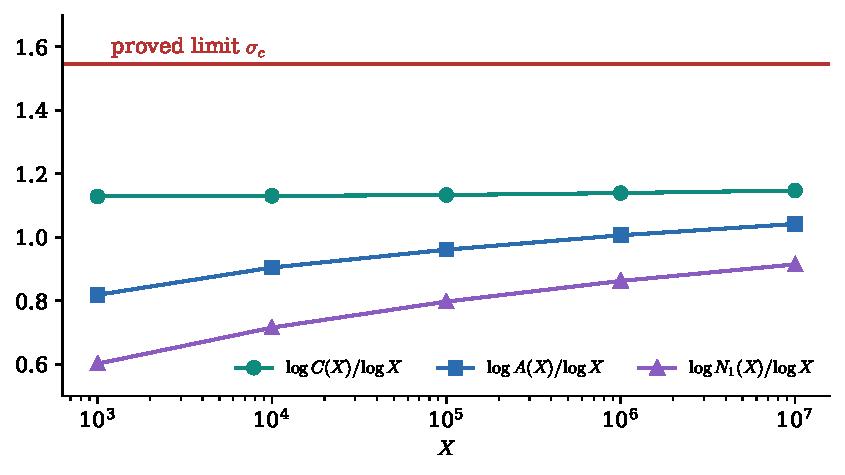
\includegraphics[width=.86\textwidth]{fig_growth.pdf}
\caption{Observed exponents against the limit of \cref{thm:growth}. Convergence is slow: at $X=10^7$ the three observed values are still well below $\sigma_c$.}\label{fig:growth}\end{figure}
\begin{figure}[htbp]\centering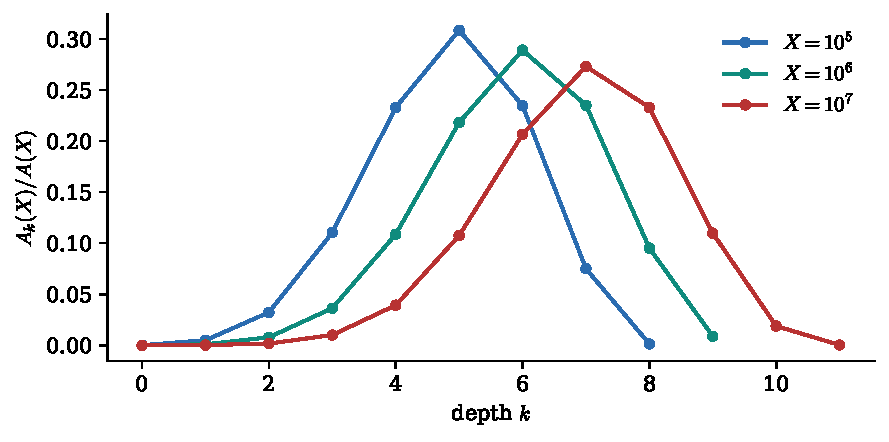
\includegraphics[width=.86\textwidth]{fig_depth.pdf}
\caption{Normalized depth distributions.}\label{fig:depth}\end{figure}
The census file lists every word with $E\le10^5$ with its record $(w,K,Q,E)$; all 63\,805 records replay from their least source. The longest word $w_p$ of \cref{lem:primes} for $p<1000$ has 15 letters.

\subsection{Factorization and prime coordinates}
All 16\,176 coprime pairs of non-squarefree integers with $mn\le10^5$ satisfy $H(mn)>H(m)H(n)$ (0 equalities, 0 reversals).
\begin{table}[htbp]\centering\small
\begin{tabular}{lrrrrr}\toprule
$f$ & $m$ & $n$ & $f(m)$ & $f(n)$ & $f(mn)$\\\midrule
$H$ & 2 & 9 & 1 & 2 & 3\\
$a$ & 2 & 9 & 0 & 1 & 1\\
$H_{1}$ & 3 & 4 & 0 & 1 & 1\\
$H_{2}$ & 2 & 9 & 0 & 0 & 1\\
$H_{3}$ & 8 & 9 & 0 & 0 & 2\\
$H_{4}$ & 9 & 32 & 0 & 0 & 3\\
$H_{5}$ & 9 & 128 & 0 & 0 & 4\\
$H_{6}$ & 9 & 512 & 0 & 0 & 5\\\bottomrule
\end{tabular}
\caption{Coprime witnesses of non-multiplicativity.}\label{tab:witness}
\end{table}
\begin{table}[htbp]\centering\small
\begin{tabular}{rrr}\toprule
$p$ & mean $v_p(E)$ & fraction with $p\mid E$\\\midrule
2 & 4.477 & 0.857\\
3 & 2.415 & 0.763\\
5 & 1.147 & 0.520\\
7 & 0.541 & 0.270\\
11 & 0.199 & 0.101\\
13 & 0.181 & 0.093\\\bottomrule
\end{tabular}
\caption{Prime coordinates of the 63\,805 words with $E\le100000$.}\label{tab:primes}
\end{table}
\subsection{Depth two and boundaries}
At $s=3$ the truncated double sum and the Hurwitz representation of \cref{thm:depth2} agree to the accuracy of the tail bound $2.3\times10^{-7}$: $0.000531393$. The partial Euler product with a tail correction gives $\kappa\approx1.85364$. Expanding the representation one order further at $s=\tfrac12$ predicts
\[A_2(X)=\sqrt X\Big(\frac\kappa2\log X+c+o(1)\Big),\qquad c=2\gamma\kappa+\tfrac12F'(\tfrac12)+S-1-\kappa,\]
where $\gamma$ is Euler's constant, $F(s)=\sum_dJ_s(d)d^{-2s}c(d)^{-2s}$ and $S=\sum_d\frac{J_{1/2}(d)}{d\,c(d)}\big(-\psi(1+\tfrac1d)-\gamma\big)$. This second term is a computed prediction and is not part of \cref{thm:depth2}; \cref{tab:A2} compares it with exact counts.
\begin{table}[htbp]\centering\small
\begin{tabular}{rrrr}\toprule
$X$ & $A_2(X)$ & gap to $c$ & gap $\times X^{1/6}$\\\midrule
$10^{5}$ & 2\,056 & 0.3763 & 2.564\\
$10^{6}$ & 8\,529 & 0.2696 & 2.696\\
$10^{7}$ & 33\,427 & 0.1771 & 2.599\\
$10^{8}$ & 126\,468 & 0.1192 & 2.569\\\bottomrule
\end{tabular}
\caption{Depth two: the gap is $A_2(X)/\sqrt X-\frac\kappa2\log X-c$ with $c=-4.5451$.}\label{tab:A2}
\end{table}
\begin{figure}[htbp]\centering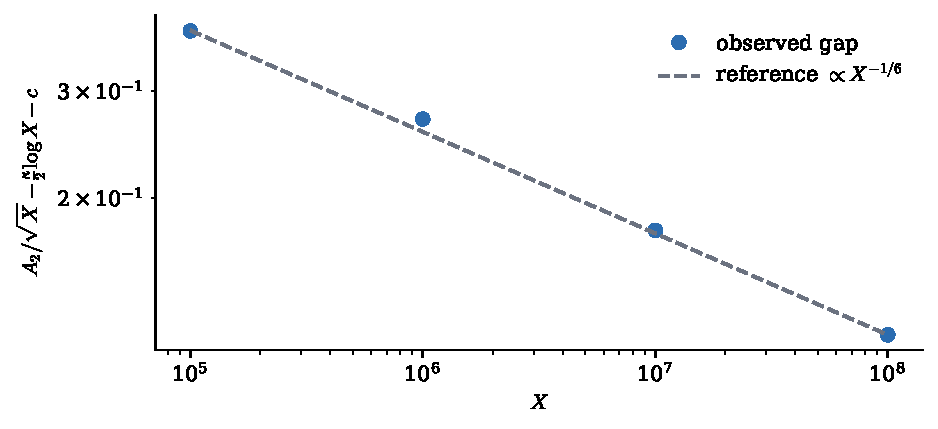
\includegraphics[width=.86\textwidth]{fig_A2.pdf}
\caption{The gap in \cref{tab:A2} and an $X^{-1/6}$ reference line.}\label{fig:A2}\end{figure}
The root $\sigma_c$ lies in $[1.54638104,\,1.54638105]$. In a sampled experiment on \cref{lem:saturation} (1000 words of length 200, labels $N\le3$), the fraction of admissible continuations rose from $0.152$ with no initial word to $1.000$ after an initial word of the largest tested size.
\subsection{Control grammars}
Both engines agree on each of the following.
\begin{table}[htbp]\centering\small
\begin{tabular}{lrrrrl}\toprule
grammar & words & endpoints & max.\ depth & boundary & $H$ witness $(m,n)$\\\midrule
$N\mapsto (N+1)^2/N$ & 9\,504 & 504 & 7 & 1.5464 & $(2,9)$\\
integer multipliers & 8\,630\,352 & 20\,000 & 14 & 1.7286 & $(2,3)$\\
square multipliers & 1\,611 & 141 & 7 & 0.8643 & $(4,9)$\\
$(N+1)^3/N$ & 153 & 60 & 4 & 0.8060 & $(4,27)$\\
prime multipliers & 431\,500 & 20\,000 & 14 & 1.3994 & $(2,3)$\\
$\{2,3\}$ & 3\,407 & 77 & 14 & 0.7879 & $(2,3)$\\
no labels & 1 & 1 & 0 & --- & none found\\
single label $N=1$ & 8 & 8 & 7 & 0.0000 & none found\\
$\{3/2,\,9/4\}$ & 143 & 10 & 9 & 0.4380 & none found\\\bottomrule
\end{tabular}
\caption{Control grammars, ceiling $20\,000$. The boundary is the abscissa of $\mathcal G(s,1)$.}\label{tab:controls}
\end{table}

\section{Further mathematical directions}
\begin{enumerate}
\item Decide convergence on the surface $|t|B(\operatorname{Re}s)=1$ and describe the singularity of
$\mathcal G(s,1)$ at $s=\sigma_c$. Does it continue beyond that point?
\item Is $A(X)=\#\{w:E(w)\le X\}$ asymptotic to $cX^{\sigma_c}$, or is there a slowly varying factor?
\item Find the region of absolute convergence of $\mathcal F(s,u,t)$ when $\operatorname{Re}(s+u)<0$.
\item Prove the second term of $A_2(X)$ and continue $G_2$ beyond $\operatorname{Re}s=1/3$.
\item For depth $k\ge3$ we conjecture $(2\sigma-1)^kG_k(\sigma)\to\kappa_k$ as $\sigma\to\tfrac12^+$, where
$\kappa_k$ is the mean of $\prod_{i=2}^k\gcd(E(N_1\cdots N_{i-1}),N_i)^{1/2}$ over independent profinitely
uniform labels; the cases $k\le2$ are proved.
\item We conjecture $H(mn)>H(m)H(n)$ for all coprime non-squarefree $m,n$. Concatenating words does not give an
injective map from pairs: for $m=4$, $n=25$ the pairs $(\varepsilon,(1,4))$ and $((1),(4))$ have the same
concatenation.
\item Classify multiplicative grammars by the limit of $G_k^{1/k}$ when the saturation hypothesis of
\cref{thm:criterion} fails.
\item Determine which statements about zeros or cancellation, if any, the continued series support.
\end{enumerate}

\appendix
\section{Register and reproduction}\label{sec:register}
\begin{center}\small
\begin{tabular}{ll}\toprule
register & statement\\\midrule
ANS-T01, T02 & \cref{thm:factor}\\
ANS-T03 & \cref{thm:evolution,cor:words}\\
ANS-T04 & \cref{thm:prime}\\
ANS-T05, T13 & \cref{thm:depth2}\\
ANS-T06 & \cref{thm:euler}\\
ANS-T07 & \cref{thm:suff}\\
ANS-T08 & \cref{thm:unit}\\
ANS-T09 & \cref{thm:sharp,cor:abscissa}\\
ANS-T10 & \cref{thm:growth}\\
ANS-T11 (partial) & \cref{thm:criterion}\\
ANS-T12 & \cref{thm:fixed}\\
ANS-T14 & \cref{thm:allhist,thm:region}\\
ANS-T15 & \cref{lem:primes,lem:saturation,thm:growth}\\
\bottomrule
\end{tabular}
\end{center}
The release directory contains the engines, a definition-level test oracle, the census files and the record file.
\texttt{python verify.py --stage E} repeats the computations (standard library only; about 1 GB of memory);
\texttt{RUN\_WINDOWS.bat} runs the smaller default stage. The batch file has not yet been executed under Windows.

\begin{thebibliography}{9}
\bibitem{monograph} UNNS Research Collective, \emph{Induced Structures in the UNNS Substrate}, Chapters 1--42,
version 1.1 (workspace release).
\bibitem{sources} UNNS Research Collective, \emph{UNNS Substrate --- Induced Structures}, source collection,
\url{https://github.com/ukbbi/UNNS/tree/d3065a0b63889286a56b3149d7724e537bd6064e/projects/UNNS_INDUCED_STRUCTURES}.
\bibitem{index} UNNS Research Collective, theorem index of the source collection,
\url{https://github.com/ukbbi/UNNS/blob/d3065a0b63889286a56b3149d7724e537bd6064e/projects/UNNS_INDUCED_STRUCTURES/THEOREM_INDEX.md}.
\bibitem{algebraic} UNNS Research Collective, \emph{Algebraic and Topological Extensions of the UNNS
Generative Law}, version 1.1, November 2026 (workspace manuscript).
\bibitem{apostol} T.~M.~Apostol, \emph{Introduction to Analytic Number Theory}, Springer, 1976.
\bibitem{delange} H.~Delange, G\'en\'eralisation du th\'eor\`eme de Ikehara,
\emph{Ann.\ Sci.\ \'Ecole Norm.\ Sup.\ (3)} \textbf{71} (1954), 213--242.
\bibitem{tenenbaum} G.~Tenenbaum, \emph{Introduction to Analytic and Probabilistic Number Theory},
Cambridge University Press, 1995.
\end{thebibliography}
\end{document}
